%%%%%%%%%%%%Outline%%%%%%%%%%%%%%%%%%

%%% section opening
%%%
% message<section three characterizes the pure-bytecode gap through three questions>
% the same program runs 1.57x (x86) and 1.98x (ARM) slower through the pipeline than native
% we characterize the gap on pure-bytecode microbenchmarks through three questions
% Q1: how much in-kernel execution slows native code
% Q2: how much an optimizing compiler recovers from the same bytecode
% Q3: which operations the kernel JIT compiles poorly

%%%
% message<the three questions decompose the gap>
% the three questions decompose the gap
% Q1 separates in-kernel execution cost from code generation quality
% Q2 weighs the per-opcode kernel JIT against the bytecode within code generation
% Q3 identifies which operations the JIT compiles poorly, to target a fix
% the section closes with why the kernel cannot host an optimizing compiler

%%% subsection Experimental Setup -- Benchmarks
%%%
% message<the benchmark corpus, computation kernels from real eBPF programs>
% 27 pure-bytecode microbenchmarks
% each a computation kernel from a real eBPF program
% examples: katran consistent-hash lookup, a SipHash-like rotation mixer
% no helpers or maps, so each measurement isolates instruction execution

%%% Experimental Setup -- Execution paths
%%%
% message<four execution paths isolate execution, JIT, and bytecode losses>
% four paths: the kernel eBPF JIT baseline plus the three in the table
% the paths vary the final backend and where the code runs
% the kernel eBPF JIT compiles the verified bytecode in the kernel, the baseline
% in-kernel and userspace native run native code inside and outside the kernel
% userspace LLVM-BPF recompiles the same bytecode with an optimizing compiler
% three pairwise comparisons attribute the gap
% in-kernel vs userspace native isolates in-kernel execution
% kernel JIT vs LLVM-BPF isolates the per-opcode kernel JIT, given the C-RQ1 bound
% LLVM-BPF vs userspace native isolates the bytecode form

%%% Experimental Setup -- Metric
%%%
% message<the speedup metric>
% a path's speedup is the kernel JIT's median time divided by the path's
% reported speedups are geometric means over the benchmarks
% load, link, compile time stay outside the speedup

%%% subsection C-RQ1
%%%
% message<in-kernel execution costs little, code generation carries the gap>
% in the kernel native code runs about as fast as in userspace
% x86: 1.55 vs 1.57, about 2 percent
% ARM: 1.88 vs 1.98, about 5 percent
% native code from the same source, differing in where the code runs
% the spread bounds in-kernel execution at about 2-5 percent
% the cost is small, the gap comes mainly from code generation

%%% subsection C-RQ2
%%%
% message<an optimizing compiler recovers most of the gap from the same bytecode>
% code from an optimizing compiler on the same bytecode runs almost as fast as native
% LLVM-BPF compiles the same verified bytecode with an optimizing backend
% LLVM-BPF reaches 1.53 (x86) and 1.92 (ARM)
% against userspace native the optimizing backend recovers 93 and 94 percent
% with execution bounded by C-RQ1, the recovered share measures the JIT loss
% the remaining 7 (x86) and 6 (ARM) percent come from the bytecode form

%%% subsection C-RQ3
%%%
% message<the JIT compiles hardware idioms poorly, shown by the rotate>
% the per-opcode kernel JIT compiles hardware idioms poorly
% an idiom has no single-instruction form, the backend spells the idiom out
% the kernel JIT translates each bytecode instruction separately
% the figure shows a variable-shift rotate under the JIT and under native compilation
% the rotate enters as eight bytecode instructions and leaves as 15
% direct native compilation uses a single rotate instruction

%%%
% message<the decomposition spans a small bounded idiom set and inflates code>
% a small bounded set of idioms expands the same way under the kernel JIT
% the rotate is one of a handful with no single-instruction form
% the table lists the idioms with instruction counts along each path
% five idiom-stress probes: the JIT emits 1.25-2.7x as many instructions as LLVM-BPF
% code size shows the cost across the whole corpus
% native code is about half the size, 0.54 (x86) and 0.49 (ARM), beyond idioms included

%%% subsection Why Not an Optimizing Compiler in the Kernel
%%%
% message<a heavy in-kernel compiler is not viable, so the simple JIT must emit idioms>
% the obvious response is an optimizing compiler in the kernel
% an in-kernel optimizing compiler would enlarge the trusted base behind the guarantee
% the verifier checks only the bytecode, the larger compiler would be trusted
% it would grow per-architecture kernel maintenance
% the practical fix keeps the simple JIT and lets the JIT emit a bounded idiom set

%%%
% message<three constraints define the fix and scope the design>
% emitting the idioms from the simple kernel JIT must meet three constraints
% the verifier must still prove every program safe
% adding an operation must not require rewriting the verifier or JIT core
% one operation maps per architecture, verification stays architecture-independent
% the fix targets the operations C-RQ3 identifies
% C-RQ1 cost and C-RQ2 residual stay out of scope, the idiom share is measured in eval

%%%%%%%%%%%%Outline%%%%%%%%%%%%%%%%%%

\section{Characterizing the Gap Between eBPF and Native Code}
\label{sec:characterization}
% eBPF 与原生性能差距的特征分析

We characterize the performance gap between eBPF and native code on microbenchmarks, small programs that only compute and make no helper calls or map accesses.
% 我们在微基准测试上特征化 eBPF 与本地代码之间的性能差距，这些是只做计算、不调用辅助函数也不访问映射的小程序。
On them, the same source program runs 1.57$\times$ faster on x86-64 and 1.98$\times$ faster on ARM64 when compiled directly to native code than through the eBPF compilation pipeline (Figure~\ref{fig:char-pure-percase}).
% 在这些基准上，同样的源程序直接编译为本地代码时，比经过 eBPF 编译管线快 1.57 倍（x86-64）和 1.98 倍（ARM64）。
The gap is consistent: native code is more than 2\% faster than the eBPF JIT's code on 25 of the 27 benchmarks on x86-64 and on all 27 on ARM64. 
% \note{[zhengjie] kernel JIT-> eBPF JIT. now there are kernel JIT / kernel eBPF JIT / eBPF JIT}
% 这一差距是一致的：本地代码在 x86-64 上 27 个基准中的 25 个、在 ARM64 上全部 27 个比eBPF JIT 快 2\% 以上。
We break the gap down through three questions:
% 我们通过三个问题分解这一差距：
\begin{itemize}
  \item \textbf{C-RQ1.} How much does in-kernel execution slow native code?
  % C-RQ1：内核内执行使原生代码慢多少？
  \item \textbf{C-RQ2.} How much of the gap can an optimizing compiler recover from the same verified bytecode?
  % C-RQ2：优化编译器能从相同的验证字节码中恢复多少差距？
  \item \textbf{C-RQ3.} Which operations does the eBPF JIT compile poorly?
  % C-RQ3：eBPF JIT 编译哪些操作效果差？
\end{itemize}

The first separates the cost of in-kernel execution from the quality of the machine code the pipeline generates.
% 第一个问题将内核内执行成本与管线生成的机器代码质量分开。
Within code generation, the second separates the eBPF JIT's share of the gap from the bytecode's.
% 在代码生成内部，第二个问题把差距中eBPF JIT 的部分和字节码的部分分开。
The third identifies which operations the JIT compiles poorly, so that a fix can target them.
% 第三个问题识别 JIT 编译效果差的操作，以便修复能够针对它们。
The section closes with why the kernel should not host an optimizing compiler (\S\ref{subsec:char-challenges}).
% 本节最后说明为什么内核不应容纳优化编译器。

\subsection{Experimental Setup}
\label{subsec:char-method}
% 实验设置

\noindent\textbf{Benchmarks.}
% \noindent\textbf{基准测试。}
We use 27 microbenchmarks, listed in Table~\ref{tab:microbenchmarks}.
% 我们使用 27 个微基准测试，见表。
Twelve of them re-implement the core computation of programs in Katran~\cite{katran}, Cilium~\cite{cilium}, BCC~\cite{bcc}, bpftrace~\cite{bpftrace}, Tetragon~\cite{tetragon}, Tracee~\cite{tracee}, and the OpenTelemetry eBPF profiler~\cite{otelprofiler}. The other fifteen are synthetic programs for packet parsing, hashing, and search.
% 其中 12 个复现了 Katran、Cilium、BCC、bpftrace、Tetragon、Tracee 和 OpenTelemetry eBPF profiler 中程序的核心计算；其余 15 个是用于包解析、哈希和搜索的合成程序。
The benchmarks make no helper calls or map accesses, so each measurement isolates instruction execution.
% 这些基准不调用辅助函数也不访问映射，因此每次测量只反映指令执行。
The gap therefore reflects only how well the pipeline translates bytecode into machine code.
In production programs, helper calls and map accesses take a larger share of the time, so the case studies in \S\ref{sec:eval} measure the end-to-end effect separately.
% 因此差距表征字节码到原生的代码生成质量；在生产程序中，辅助和映射时间稀释指令执行份额，所以案例研究单独测量端到端效果。

\noindent\textbf{Execution paths.}
% \noindent\textbf{执行路径。}
We run each benchmark through four execution paths that differ in which compiler produces the machine code and where the code runs.
% 我们让每个基准测试经过四条执行路径，它们在由哪个编译器生成机器代码以及代码在哪里运行上有所不同。
The eBPF JIT compiles the verified bytecode in the kernel and is the baseline.
% eBPF JIT 在内核中编译验证后的字节码，是基线。
In-kernel native and userspace native compile the C source directly to native code and run it inside and outside the kernel, respectively.
% 内核内原生和用户空间原生将 C 源代码直接编译为本地代码，分别在内核内和内核外运行。
Userspace LLVM-BPF recompiles the same bytecode with an optimizing compiler in userspace~\cite{zheng2025extending}.
% 用户空间 LLVM-BPF 使用用户空间的优化编译器重新编译相同的字节码。
Three pairwise comparisons attribute the gap.
% 三个成对比较归因差距。
In-kernel native against userspace native isolates in-kernel execution.
% 内核内原生与用户空间原生对比隔离内核内执行。
The eBPF JIT against userspace LLVM-BPF isolates the eBPF JIT's code generation.
% eBPF JIT 与用户空间 LLVM-BPF 对比，在 C-RQ1 表明在内核中运行代价很小之后，隔离出eBPF JIT 的代码生成。
Userspace LLVM-BPF against userspace native isolates the bytecode itself.
% 用户空间 LLVM-BPF 与用户空间原生对比隔离字节码本身。

\noindent\textbf{Metric.}
% \noindent\textbf{度量。}
A path's speedup on a benchmark is the eBPF JIT's median steady-state execution time divided by the path's time.
% 一条路径在基准测试上的加速比是eBPF JIT 的中位稳态执行时间除以该路径的时间。
Each reported speedup is the geometric mean over the benchmarks.
% 每个报告的加速比是所有基准测试的几何平均值。
Load, link, and compile time stay outside the speedup.
% 加载、链接和编译时间不计入加速比。

% \begin{table}[t]
\centering
\small
\caption{Speedup over the kernel eBPF JIT on the 27 pure-bytecode microbenchmarks, as the geometric mean of median steady-state time. A path counts as faster on a benchmark when it beats the kernel eBPF JIT by more than 2\%.}
\label{tab:char-micro-summary}
\begin{tabular}{@{}llcc@{}}
\toprule
Platform & Path & Speedup & \# Cases Faster \\
\midrule
x86-64 & In-kernel native   & 1.55$\times$ & 24/27 \\
       & Userspace native   & 1.57$\times$ & 25/27 \\
       & Userspace LLVM-BPF & 1.53$\times$ & 25/27 \\
\midrule
ARM64  & In-kernel native   & 1.88$\times$ & 27/27 \\
       & Userspace native   & 1.98$\times$ & 27/27 \\
       & Userspace LLVM-BPF & 1.92$\times$ & 27/27 \\
\bottomrule
\end{tabular}
\end{table}
\begin{table*}[t]
\centering
\small
\caption{Computational microbenchmarks used in Figure~\ref{fig:char-pure-percase}. Benchmarks with a citation re-implement the core computation of that production program; the other 15 are synthetic. The \texttt{cksum} and \texttt{tc\_cksum} programs perform the same computation with different eBPF program types.}
\label{tab:microbenchmarks}
\renewcommand{\arraystretch}{1.08}
\begin{tabular*}{\textwidth}{@{\extracolsep{\fill}}ll@{\hspace{1.2em}}ll@{\hspace{1.2em}}ll@{}}
\toprule
\textbf{Benchmark} & \textbf{Computation} & \textbf{Benchmark} & \textbf{Computation} & \textbf{Benchmark} & \textbf{Computation} \\
\midrule
\texttt{bitmap} & Bit counting, mixing & \texttt{katran} & Hash-based selection~\cite{katran} & \texttt{sock\_lb} & Service selection~\cite{cilium} \\
\texttt{bin\_search} & Sorted-rule binary search & \texttt{policy} & Nested conditions~\cite{cilium} & \texttt{tcpconn} & Connection filtering~\cite{bcc} \\
\texttt{runqlat} & Logarithmic buckets~\cite{bcc} & \texttt{siphash} & SipHash-style mixing & \texttt{tetragon} & Process-event filtering~\cite{tetragon} \\
\texttt{trace\_sw} & Switch dispatch & \texttt{bounds} & Bounds checks, reads & \texttt{otel} & Frame-record scan~\cite{otelprofiler} \\
\texttt{cksum} & Checksum & \texttt{field} & Field reads, mixing & \texttt{ct\_nat} & Address rewriting~\cite{cilium} \\
\texttt{memcmp} & Bytewise comparison & \texttt{bitfield} & Bit-field extraction & \texttt{toeplitz} & Toeplitz-style hashing \\
\texttt{vlan} & Packet-header parsing & \texttt{str\_search} & Substring search~\cite{bpftrace} & \texttt{fnv} & FNV-1a hashing~\cite{bpftrace} \\
\texttt{call\_fanout} & Local-call dispatch & \texttt{syscall} & Syscall name lookup~\cite{tracee} & \texttt{tc\_cksum} & Checksum (TC) \\
\texttt{5tuple} & Jenkins-style hashing & \texttt{http} & HTTP prefix detection~\cite{tracee} & \texttt{cgroup} & Hash mixing \\
\bottomrule
\end{tabular*}
\end{table*}


\subsection{C-RQ1: How Much Does In-Kernel Execution Slow Native Code?}
\label{subsec:gap}
% C-RQ1：内核内执行使原生代码慢多少？

In the kernel, native code runs about as fast as in userspace.
% 在内核中，原生代码运行速度与用户空间大致相同。
In-kernel native and userspace native run the same native code and differ only in where it runs.
% 内核内原生和用户空间原生运行相同的本地代码，只在运行位置上不同。
On x86-64, Figure~\ref{fig:char-pure-percase} shows them at 1.55$\times$ and 1.57$\times$ over the eBPF JIT, a difference of about 2\%. On ARM64 the difference is about 5\%, 1.88$\times$ against 1.98$\times$.
% 在 x86-64 上，图显示二者相对eBPF JIT 分别为 1.55 倍和 1.57 倍，差异约 2\%；在 ARM64 上差异约 5\%，1.88 倍对 1.98 倍。
This difference therefore bounds the cost of in-kernel execution at about 2--5\%.
% 因此这一差异将内核内执行的代价限定在约 2--5\%。
The cost is small, and the gap comes mainly from code generation.
% 成本很小，差距主要来自代码生成。

\begin{finding}
\finlabel The gap between eBPF and native code comes from code generation. In-kernel execution slows native code by only about 2\% on x86-64 and 5\% on ARM64.
% 发现：eBPF 与原生的差距来自代码生成。内核内执行仅使原生代码在 x86-64 上慢约 2\%，在 ARM64 上慢约 5\%。
\end{finding}

\begin{figure*}[t]
\centering
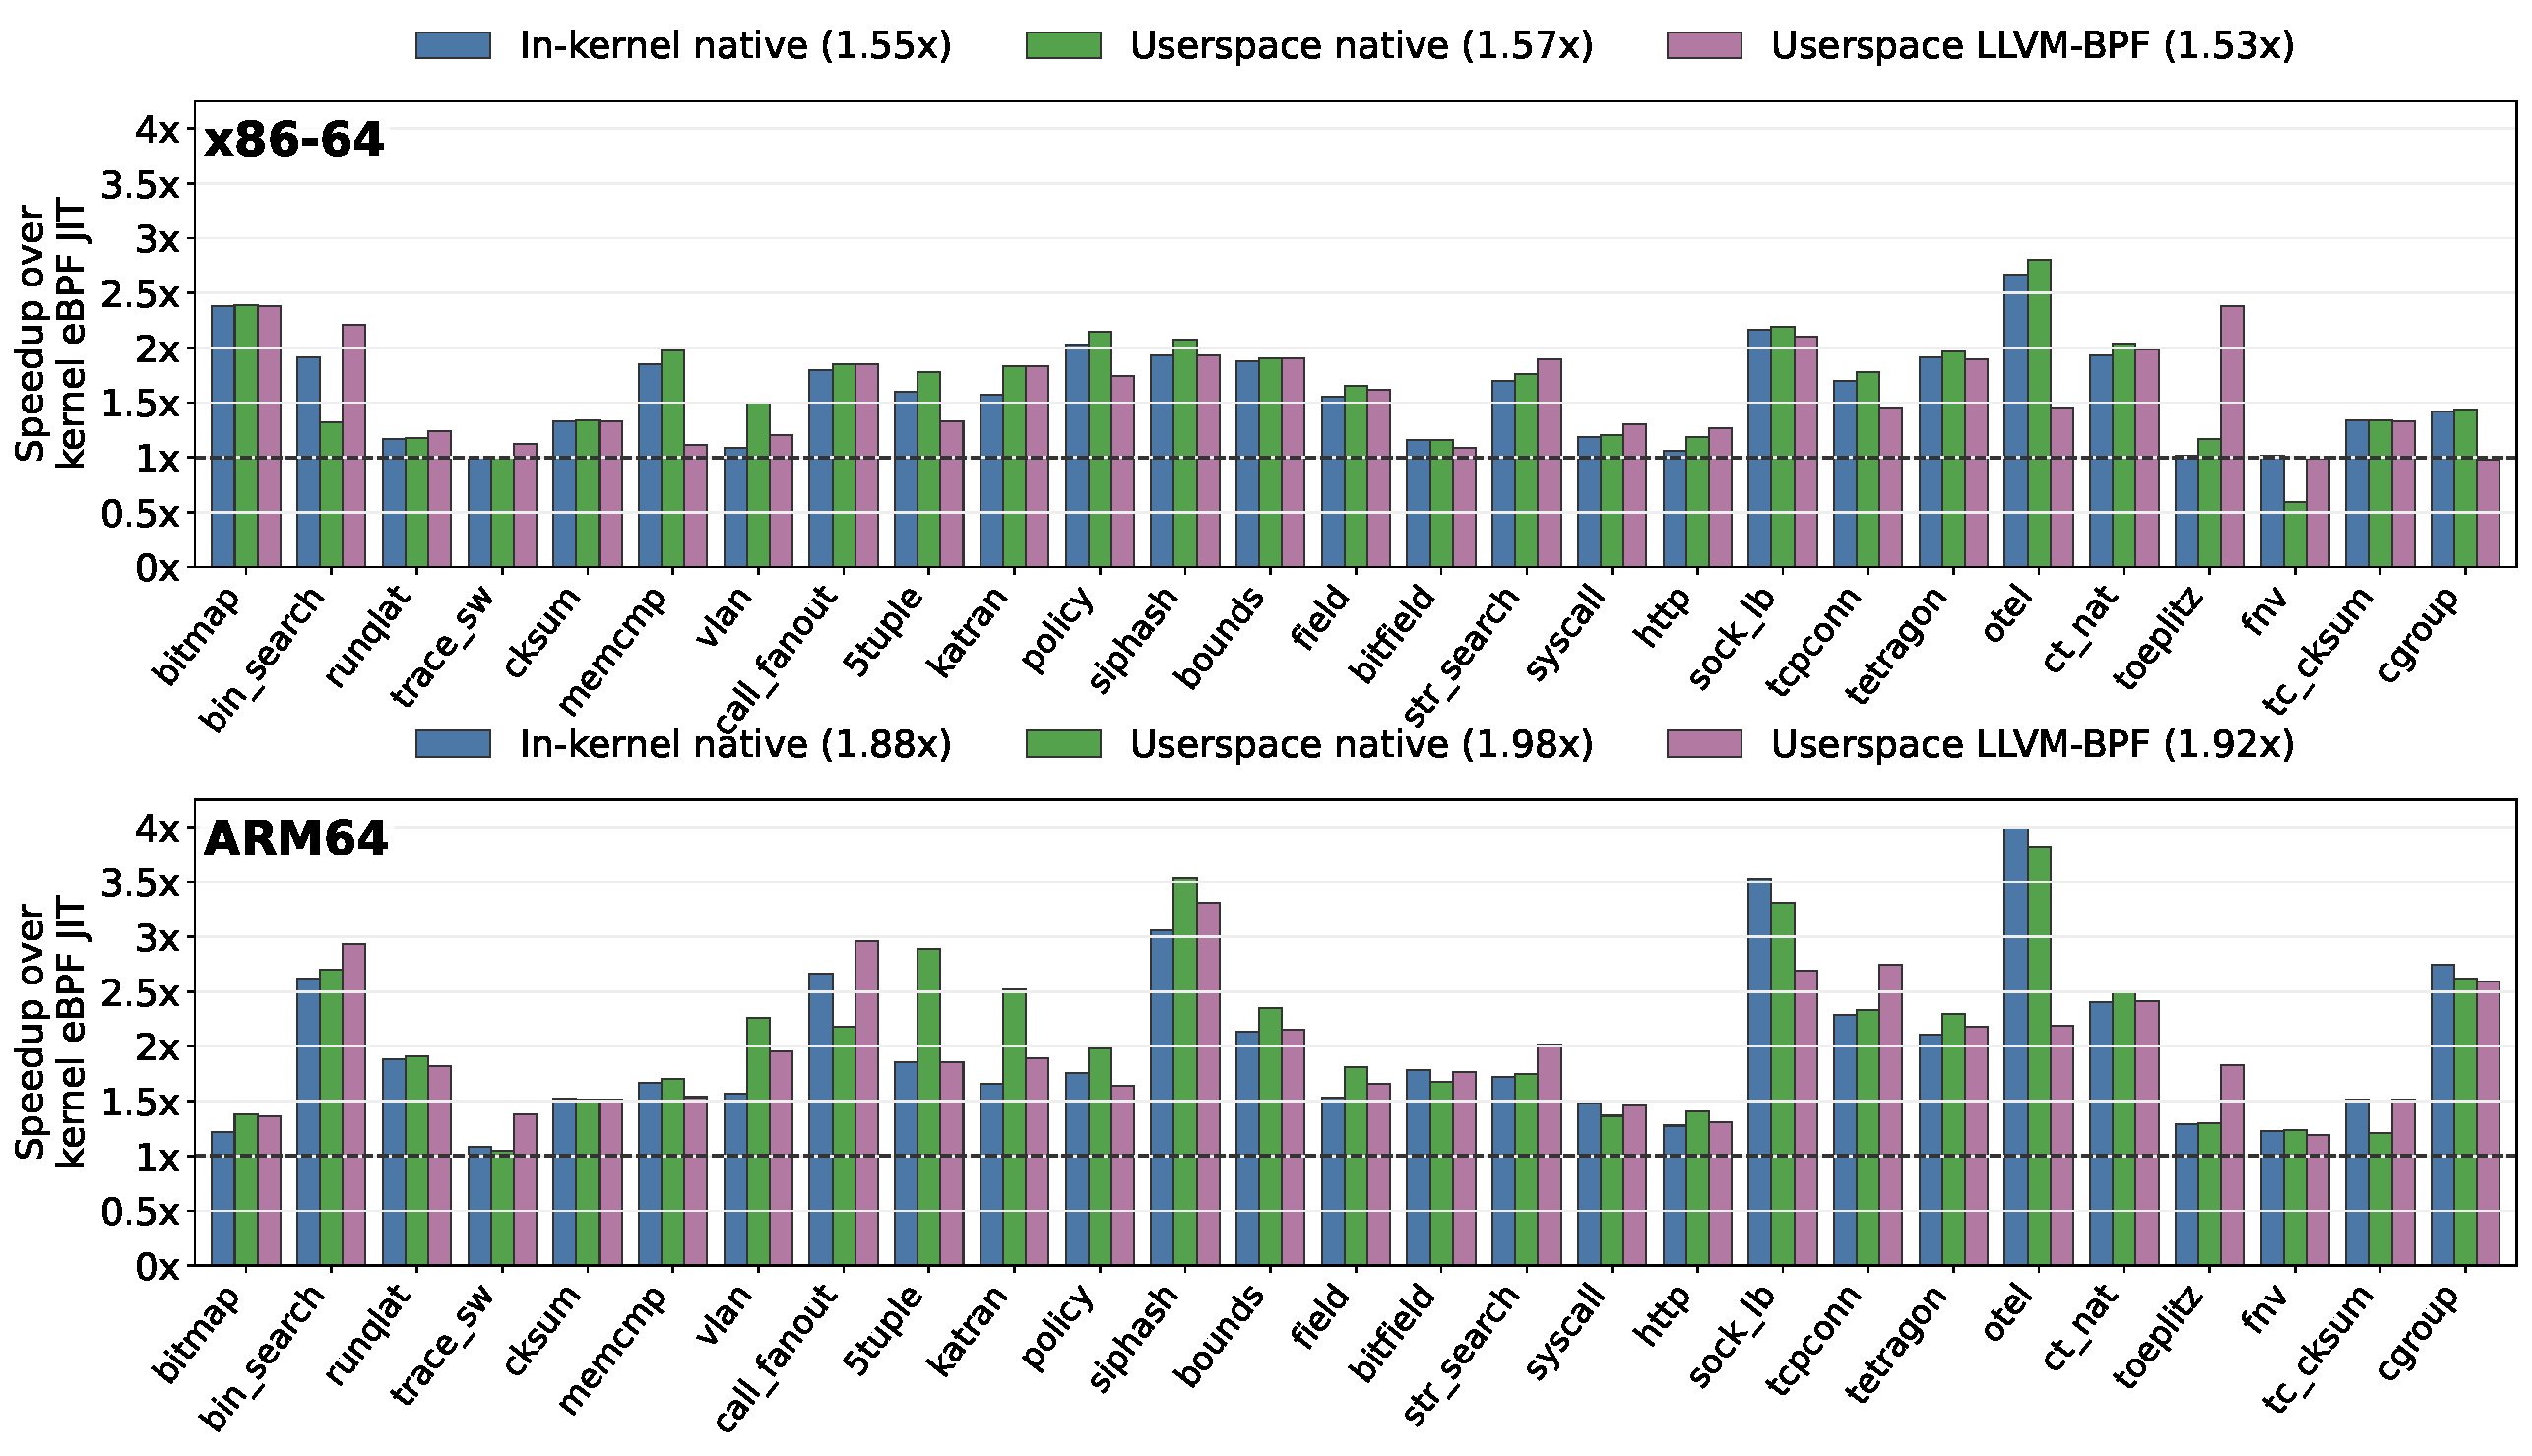
\includegraphics[width=\textwidth]{figures/sec-3-4config-percase.pdf}
\caption{Per-case speedup over the kernel eBPF JIT on the 27 microbenchmarks, on x86-64 (top) and ARM64 (bottom). Each bar is one non-baseline path. The ARM64 paths come from separate runs, each over its own baseline.}
\label{fig:char-pure-percase}
\end{figure*}


\subsection{C-RQ2: How Much Can an Optimizing Compiler Recover?}
\label{subsec:char-jit}
% C-RQ2：优化编译器能恢复多少？

Code from an optimizing compiler on the same bytecode runs almost as fast as native code.
% 对相同字节码应用优化编译器生成的代码运行速度几乎与原生代码相同。
Userspace LLVM-BPF compiles the same verified bytecode that the kernel runs, but with an optimizing compiler in place of the eBPF JIT.
% 用户空间 LLVM-BPF 编译内核运行的相同验证字节码，但用优化编译器替代eBPF JIT。
As Figure~\ref{fig:char-pure-percase} shows, userspace LLVM-BPF reaches 1.53$\times$ on x86-64 and 1.92$\times$ on ARM64.
% 如表所示，用户空间 LLVM-BPF 在 x86-64 上达到 1.53 倍，在 ARM64 上达到 1.92 倍。
Against userspace native at 1.57$\times$ and 1.98$\times$, it recovers 93\% and 94\% of the gap.
% 对比用户空间原生的 1.57 倍和 1.98 倍，它恢复了 93\% 和 94\% 的差距。
Because C-RQ1 shows that running in the kernel costs little, the recovered share measures the performance the eBPF JIT loses.
% 由于 C-RQ1 表明在内核中运行代价很小，恢复的份额衡量的是eBPF JIT 损失的性能。
The remaining share of the gap, 7\% on x86-64 and 6\% on ARM64, comes from the bytecode itself, which fixes choices such as the register set and calling convention before any compiler runs.
% 剩余的差距份额，x86-64 上 7\%，ARM64 上 6\%，来自字节码形式，它在任何编译器运行前固定了寄存器集和调用约定等选择。

\begin{finding}
\finlabel The eBPF JIT causes most of the gap. An optimizing compiler recovers 93--94\% of the gap from the same verified bytecode. The verified bytecode carries most of what a compiler needs to generate fast code.
% 发现：eBPF JIT 造成了大部分差距。优化编译器从相同的验证字节码中恢复 93--94\% 的差距。验证字节码携带了编译器生成快速代码所需的大部分信息。
\end{finding}

\subsection{C-RQ3: Which Operations Does the eBPF JIT Compile Poorly?}
\label{subsec:char-idiom}
% C-RQ3：eBPF JIT 编译哪些操作效果差？

The eBPF JIT compiles hardware idioms poorly.
% eBPF JIT 编译硬件习语效果差。
A hardware idiom has no single-instruction form in the eBPF instruction set, so the eBPF backend emits the idiom as several bytecode instructions (\S\ref{sec:background}).
% 硬件习语在 eBPF 指令集中没有单指令形式，因此 eBPF 后端将习语发射为多条字节码指令。
The eBPF JIT then translates each bytecode instruction separately into one or more machine instructions.
% 然后eBPF JIT 将每条字节码指令单独翻译为一条或多条机器指令。
Figure~\ref{fig:jit-dump} shows a 64-bit rotate with a variable shift under the eBPF JIT and when compiled directly to native code.
% 图显示了 64 位可变位移旋转在eBPF JIT 下和直接编译为本地代码时的情况。
The rotate arrives at the eBPF JIT as eight bytecode instructions and is emitted as 15 machine instructions.
% 旋转以 8 条字节码指令到达eBPF JIT，被发射为 15 条机器指令。
Compiled directly to native code, the rotate becomes a single instruction, \texttt{ROL} on x86-64 or \texttt{ROR} on ARM64.
% 直接编译为本地代码时，旋转只是一条指令，x86-64 上是 ROL，ARM64 上是 ROR。

\begin{figure}[t]
  \centering
  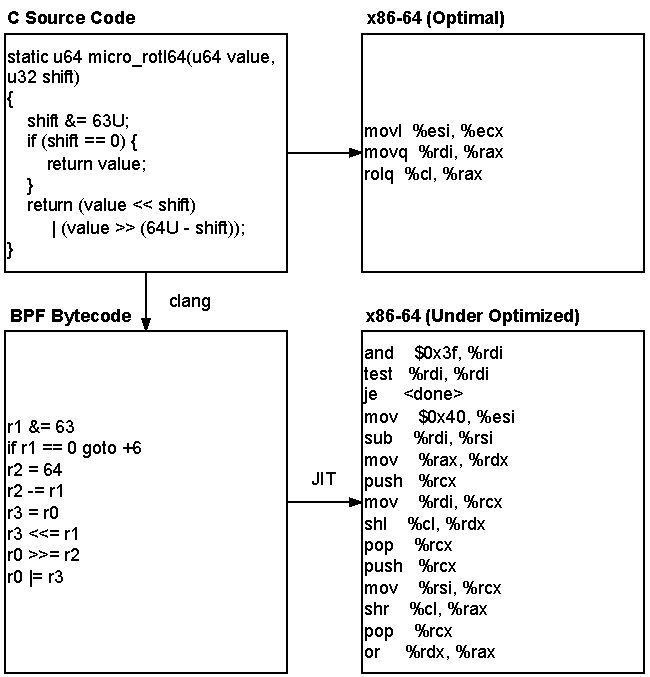
\includegraphics[width=\linewidth]{figures/sec-3-jit-dump-fig.pdf}
  \caption{Compiling a 64-bit rotate with a variable shift for x86-64, directly and through eBPF and the Linux 6.1 eBPF JIT.}
  \label{fig:jit-dump}
\end{figure}



The rotate is one of a small set of hardware idioms that expand the same way under the eBPF JIT.
% 旋转是一小组硬件习语之一，它们在eBPF JIT 下以相同方式展开。
Table~\ref{tab:isa-gap} lists the idioms with their instruction counts in native code, in eBPF bytecode, and after the eBPF JIT.
% 表列出了这些习语，以及它们在本地代码、eBPF 字节码和eBPF JIT 输出中的指令数。
Across five small test programs on x86-64 that each repeat one idiom, the eBPF JIT emits 1.25--2.7$\times$ as many instructions as userspace LLVM-BPF for the same programs.
% 在 x86-64 上的五个小测试程序中，每个程序重复一种习语，eBPF JIT 发射的指令是用户空间 LLVM-BPF 的 1.25--2.7 倍。
Code size shows how much the eBPF JIT inflates code across all 27 benchmarks.
% 代码大小显示了eBPF JIT 在全部 27 个基准上把代码膨胀了多少。
In-kernel native machine code is about half the size of the eBPF JIT output, 0.54$\times$ on x86-64 and 0.49$\times$ on ARM64, an aggregate that includes losses beyond the idioms.
% 内核内原生机器代码大约是eBPF JIT 输出的一半大小，x86-64 上 0.54 倍，ARM64 上 0.49 倍，这一汇总包括习语之外的损失。

\begin{finding}
\finlabel A significant share of the eBPF JIT's loss comes from a small set of hardware idioms, such as rotate, multi-byte load, and conditional select. The remaining loss comes from cross-instruction optimizations, such as register allocation and instruction scheduling, that are outside the scope of a per-idiom fix.
% 发现：eBPF JIT 损失的很大一部分来自一小组硬件习语，如旋转、多字节加载和条件选择。剩余损失来自跨指令优化，如寄存器分配和指令调度，这超出了逐习语修复的范围。
\end{finding}

\begin{table}[t]
\centering
\small
\caption{Hardware idioms and their instruction counts along each path, measured on x86-64 from real JIT dumps and compiler output. The second column names the native instruction on x86-64 / ARM64. Byte swap assumes a \texttt{MOVBE}-capable x86-64. The bulk-copy row is a 64-byte copy between non-overlapping regions.}
\label{tab:isa-gap}
\setlength{\tabcolsep}{3pt}
\resizebox{\columnwidth}{!}{%
\begin{tabular}{@{}llccc@{}}
\toprule
 & & \multicolumn{3}{c}{\# Instructions} \\
\cmidrule(lr){3-5}
Operation & Native instruction & Native & eBPF & eBPF JIT \\
\midrule
Rotate & \texttt{ROL}/\texttt{ROR} & 1 & 8 & 15 \\
Multi-byte load & \texttt{MOV}/\texttt{LDR} & 1 & 22 & 22 \\
Conditional select & \texttt{CMP+CMOV}/\texttt{CMP+CSEL} & 2 & 3 & 4 \\
Byte swap & \texttt{MOVBE}/\texttt{REV} & 1 & 2 & 2 \\
Bulk copy (64\,B) & \texttt{MOVUPS}/\texttt{LDP+STP} & 4 & 16 & 16 \\
\bottomrule
\end{tabular}}
\end{table}

\subsection{Why Not an Optimizing Compiler in the Kernel?}
\label{subsec:char-challenges}
% 为什么不在内核中使用优化编译器？

An obvious way to recover this loss is to replace the eBPF JIT with an optimizing compiler.
% 追回这部分损失的一个明显方法是用优化编译器替换eBPF JIT。
An optimizing compiler in the kernel would enlarge the trusted computing base behind eBPF's safety guarantee.
% 内核中的优化编译器会扩大 eBPF 安全保证背后的可信计算基。
The verifier checks only the bytecode, so the kernel would have to trust the far larger compiler that produces the native code.
% 验证器只检查字节码，因此内核必须信任生成原生代码的更大编译器。
Such a compiler would also grow the kernel code that must be maintained and audited for each supported architecture.
% 这样的编译器还会增加每个支持架构必须维护和审计的内核代码。
A practical fix instead keeps the simple eBPF JIT and targets the share of the loss that comes from hardware idioms by letting the JIT emit hardware idioms directly.
% 实际的修复方案是保持简单的eBPF JIT，通过让 JIT 直接发射硬件习语来针对损失中的习语份额。

\S\ref{sec:mechanism} presents a design that achieves this fix.
% \S\ref{sec:mechanism} 给出实现这一修复的设计。
The in-kernel execution cost (C-RQ1) and the share of the gap due to the bytecode itself (C-RQ2) stay out of scope, and \S\ref{sec:eval} measures how much of the eBPF JIT's loss the idioms carry.
% 内核内执行代价（C-RQ1）和由字节码本身造成的那部分差距（C-RQ2）不在范围内，评估测量习语承载了多少eBPF JIT 的损失。